\subsection{Software} \label{sec:Software}
\textit{(pro)} Die Software des Planting Robots ist in der Programmiersprache C geschrieben und läuft auf dem ARM Cortex M0+ Mikrocontroller von NXP welcher auf dem FRDM-Board KL25Z bestückt ist. Für low Level Driver werden diverse Processor Expert Komponenten verwendet. Als Betriebssystem dient das Real Time OS FreeRTOS. Vorteile von FreeRTOS gegenüber anderen C Betriebssystemen sind:

\begin{itemize}
	\item Seine geringen Ressourcenanforderungen an RAM, ROM und CPU Leistung. 
	\item FreeRTOS ist weit verbreitet und wird an der HSLU in diversen Softwareprojekten verwendet.
	\item Es ist absolut kostenfrei, auch für kommerzielle Anwendungen.
	\item FreeRTOS ist einfach in der Anwendung, eignet sich jedoch auch für grössere Projekte.
\end{itemize}

In den folgenden Unterkapiteln werden die wichtigsten Softwarekomponenten des Planting Robots beschrieben und erklärt. Die Titel der Unterkapitel korrespondieren dabei mit den Namen der .c Files des Codes im Anhang.

\subsubsection{FSM} \label{sec:FSM}
Der Planting Robot wird durch einen endlichen Zustandsautomaten FSM gesteuert. Die Zustände oder States die FSM sind in Abb. \ref{fig:FSM} illustriert. Ein State Wechsel wird entweder durch eine User Eingabe übe das HMI, eine Topferkennung durch den IR-Sensor oder durch fertigstellen eines States ausgeführt. Im folgenden Abschnitt werden die verschiedenen States sowie State-Wechsel erklärt:

\begin{figure}[H]
	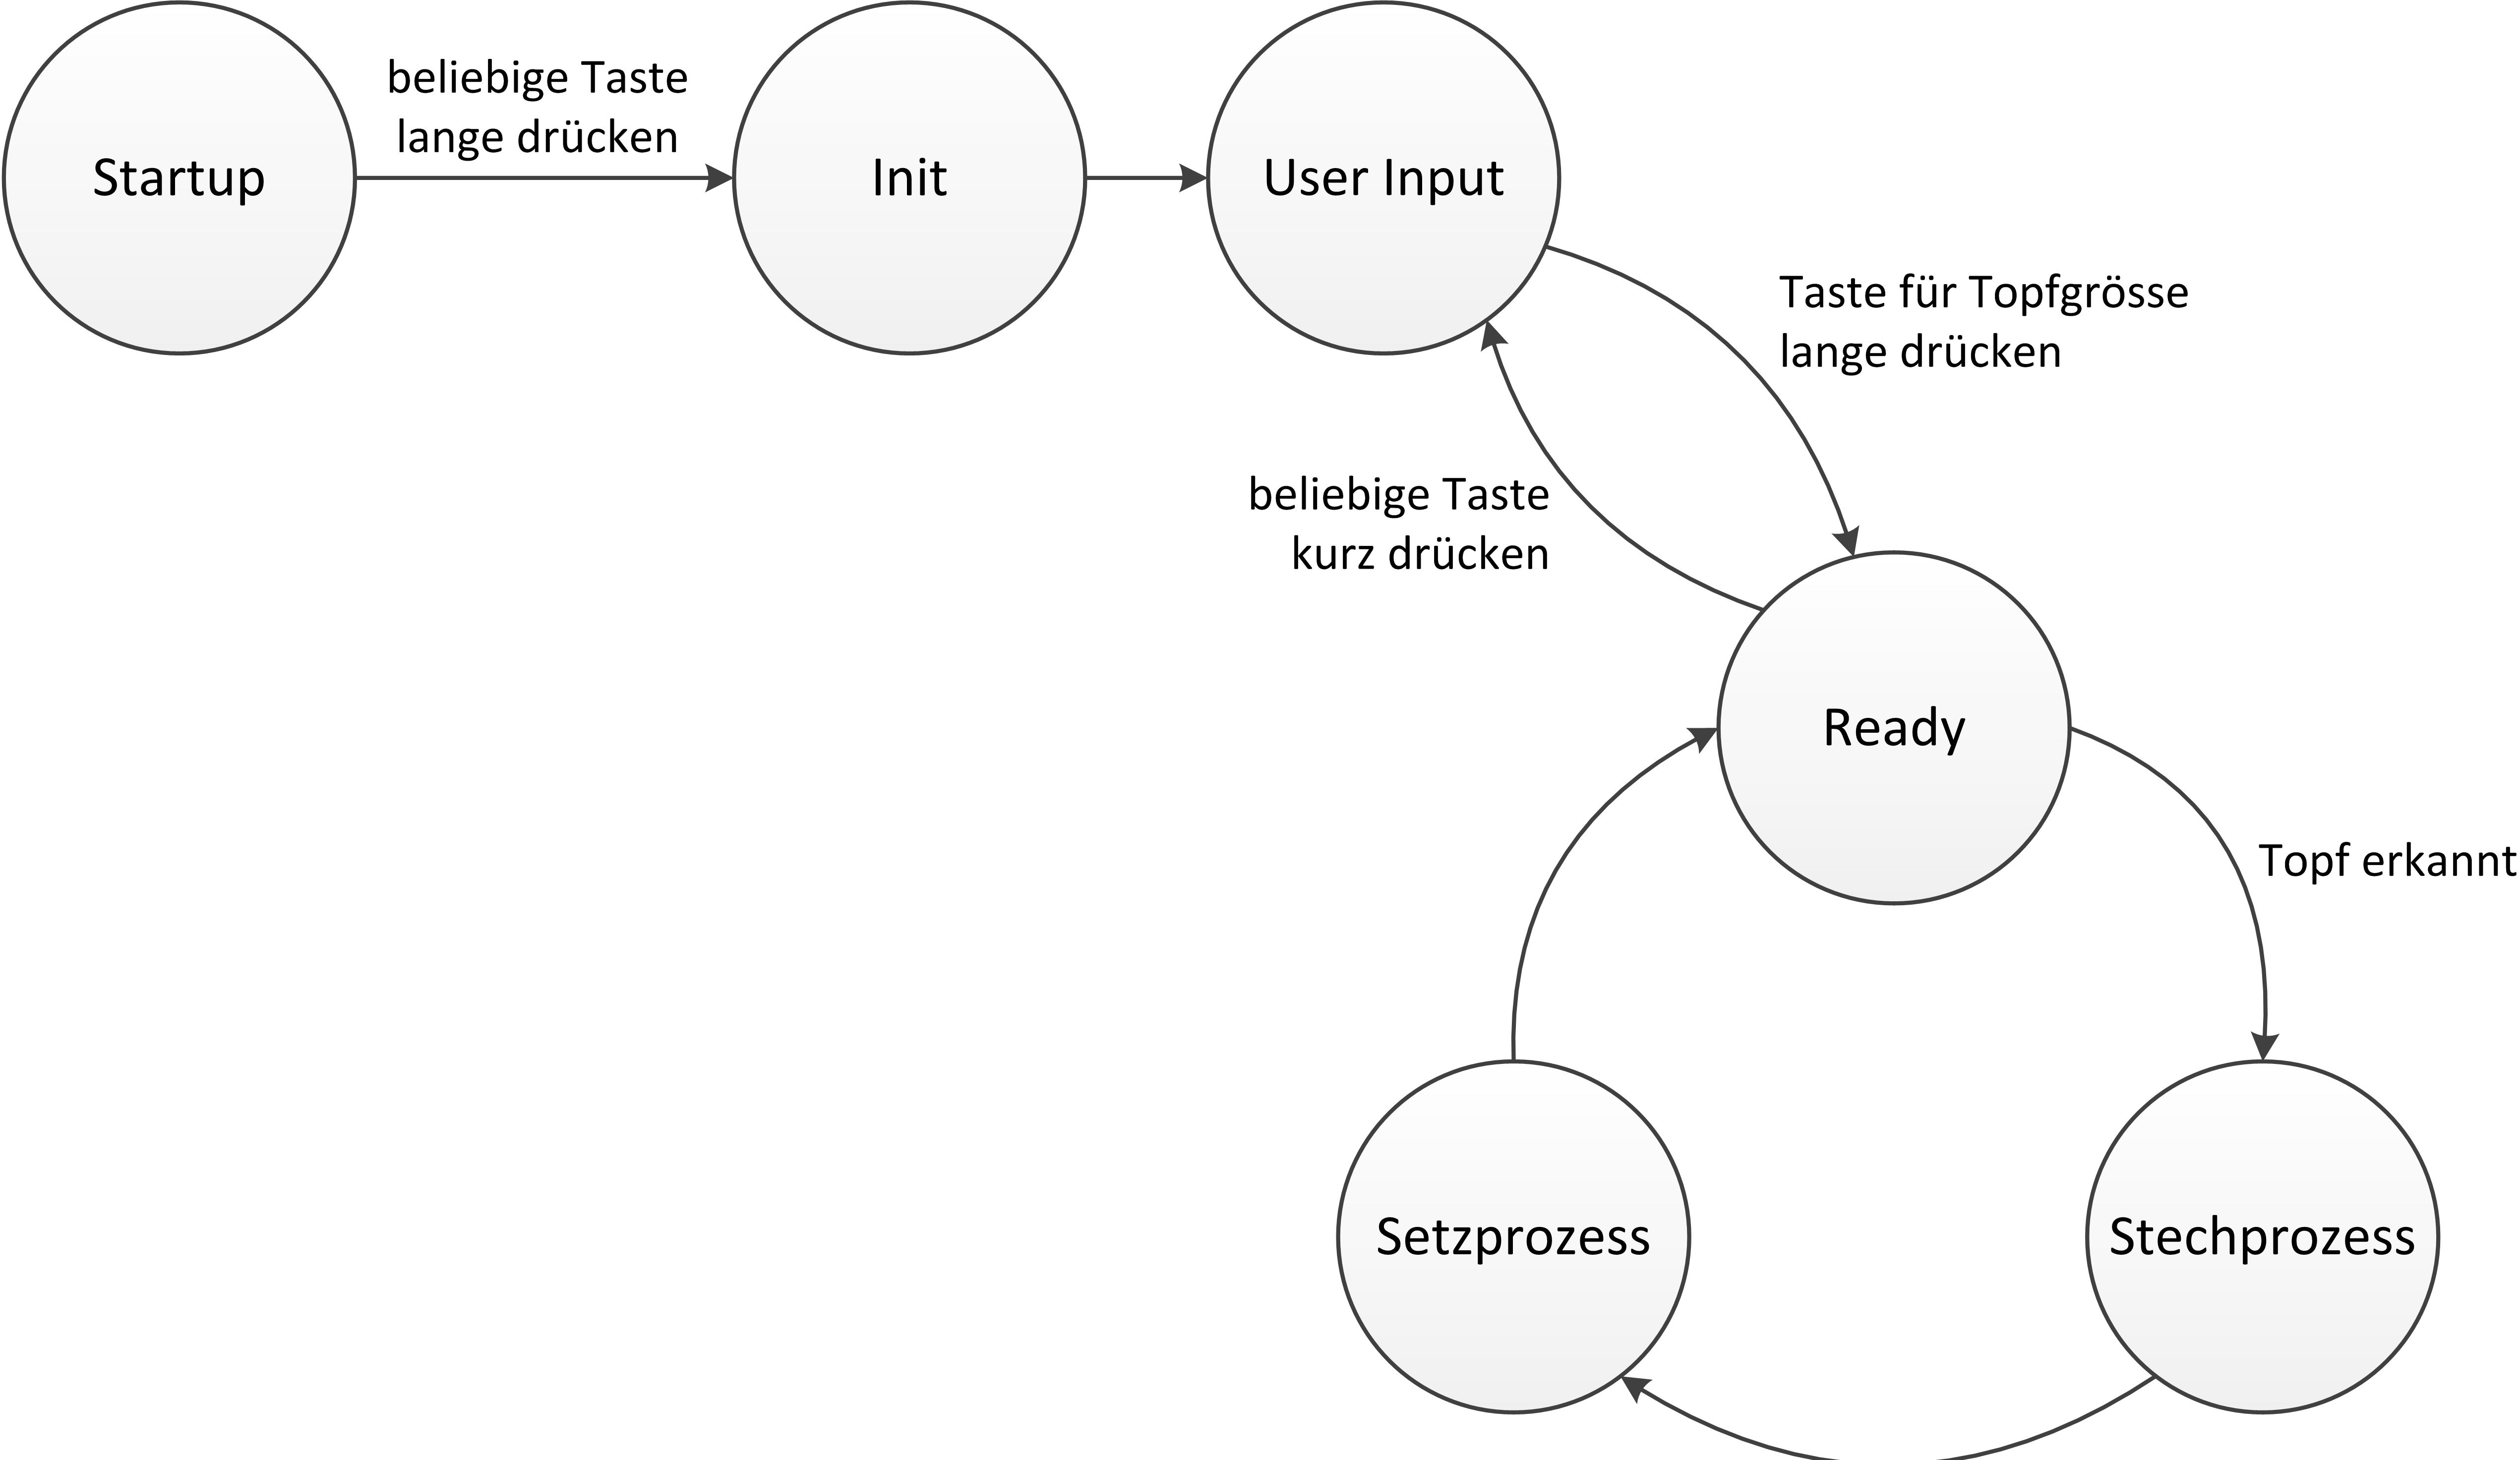
\includegraphics[width=0.9\textwidth]{Illustrationen/6-Umsetzung/FSM_B&W_breit.png}
	\caption{Software, FSM}
	\label{fig:FSM}
\end{figure}

\textbf{Startup:} Wenn die Speisung zum uC eingeschaltet wird, begibt sich die Software in den sicheren Zustand $"$Startup$"$. In diesem State sind sämtliche Aktoren stromlos. Alle LEDs des HMIs pulsieren synchron. Wird ein beliebiger Taster des HMIs länger als eine halbe Sekunde gedrückt wechselt die Software in den $"$Init$"$ State.\\
\newline
\textbf{Init:} In diesem State werden die Motoren für die Vereinzelung, die Verstellmechanik und die Setzeinheit initialisiert. Da die Motoren über Drehencoder und nicht über absolute Positionsencoder verfügen, müssen diese zuerst in ihre Ausgangsposition gebracht werden. Der Initialisierungsprozess zu den jeweiligen Motoren wird in den Kapiteln \ref{sec:Vereinzelung}, \ref{sec:Setzeinheit} und \ref{verstellmechanik} erklärt. Während der Initialisierung blinken die HMI LEDs des jeweiligen Prozesses. Nach Abschluss der Initialisierung wechselt die State Machine in den $"$User Input$"$ State.\\
\newline
\textbf{User Input:} Dieser State dient zur Konfiguration des Planting Robots. Der Operator kann hier die Topfgrösse des aktuellen Batches und die Setztiefe der Nemacaps über das HMI einstellen. Ausserdem kann der Planting Robot in diesem State manuell über die Tasten $"$manuelle Steuerung$"$ bedient werden. Mehr zur manuellen Steuerung ist im Kapitel \ref{sec:HMI} nachzulesen. Um die Konfiguration zu speichern und den Planting Robot in Betrieb zu setzen muss der Taster für die gewünschte Topfgrösse lange gedrückt werden.\\
\newline
\textbf{Ready:} Der Planting Robot befindet sich im regulären Betriebsmodus. Sobald ein Topf erkannt wird, verrichtet der Planting Robot seine Arbeit indem er den Stechprozess und anschliessend den Setzprozess ausführt. Um den Planting Robot zu stoppen, kann ein beliebiger Taster gedrückt werden. Der Planting Robot wechselt dann zurück in den $"$User Input$"$ State.\\
\newline
\textbf{Stechprozess:} Dieser Prozess wird durchlaufen sobald ein Topf erkannt wurde. Dabei wird mit dem Spindelantrieb eine Hubbewegung ausgeführt bei welcher der Stechdorn in die Erde gedrückt und wieder angehoben wird.\\
\newline
\textbf{Setzprozess:} Sobald der Stechprozess beendet ist wird der Setzprozess ausgeführt. Dabei wird die Vereinzlung angetrieben, sodass NemaCaps vom Schüttgutlager in die Topferde befördert wird. Nach beenden des Setzprozesses geht die FSM wieder in den $"$Ready$"$ State.

\subsubsection{HMI Driver}
Im HMI\_Driver.c File wird der HMI\_Task erzeugt. Alle 10ms führt dieser den Debounce Prozess aus. Dabei wird die Funktion FunktionKEYDBNC\_Process() aufgerufen, welche den Status aller Taster des HMIs ausliest und über eine State Machine entprellt. Der Debounce Prozess generiert dann ein Event für jeden Tastendruck, langen Tastendruck und loslassen eines Tasters. Events werden vom Event.c File in einem Event Array abgespeichert. Es wird somit ein Polling der HMI Taster mit einer Frequenz von 100Hz durchgeführt. Diese Programmsequenz ist in Abb. \ref{fig:Taster_Polling} oben grafisch dargestellt.


\begin{figure}[H]
	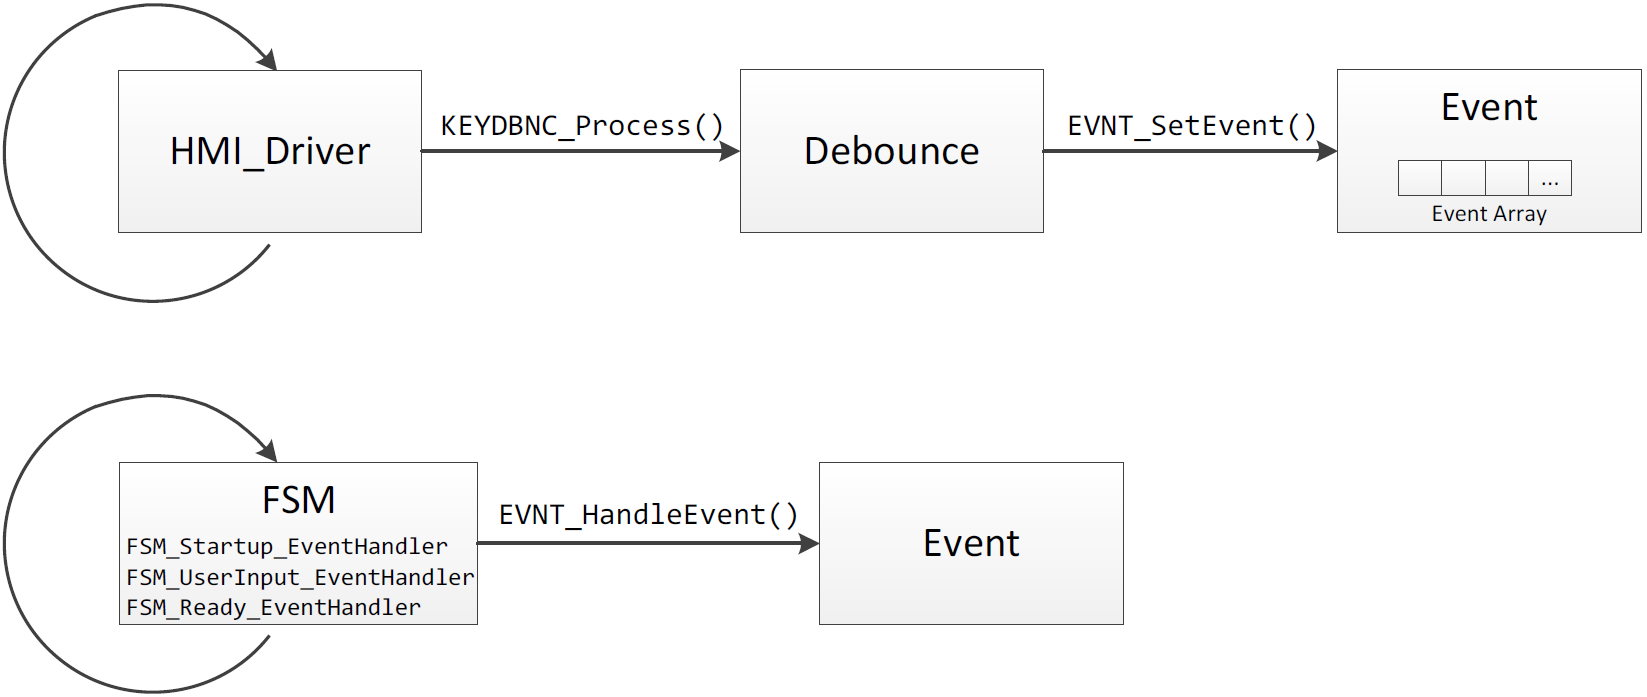
\includegraphics[width=0.9\textwidth]{Illustrationen/6-Umsetzung/Taster_Polling.png}
	\caption{Software, Taster Polling / Auswertung}
	\label{fig:Taster_Polling}
\end{figure}

Der untere Teil der Grafik in Abb. \ref{fig:Taster_Polling} beschreibt die Auswertung eines Tastendrucks. Dazu werden die vom Debounce Prozess erzeugte Events in einem der drei Eventhandler (FSM\_Startup\_EventHandler, FSM\_UserInput\_EventHandler oder FSM\_Ready\_EventHandler) des FSM.c Files ausgewertet. Eine solche Taster Event Auswertung ist am Beispiel des FSM\_Startup\_EventHandler im folgenden Code dargestellt:

\begin{lstlisting}
void FSM_Startup_EventHandler(EVNT_Handle event) {
	switch(event) {
		case EVNT_BTN_9cm_LPRESSED:				// Any Button Long Press
		case EVNT_BTN_11cm_LPRESSED:
		case EVNT_BTN_12cm_LPRESSED:
		case EVNT_BTN_13cm_LPRESSED:
		case EVNT_BTN_14cm_LPRESSED:
		case EVNT_BTN_AUTO_LPRESSED:
		case EVNT_BTN_Setzeinheit_runter_LPRESSED:
		case EVNT_BTN_Setzeinheit_hoch_LPRESSED:
		case EVNT_BTN_Vereinzelung_LPRESSED:
		case EVNT_BTN_hoeher_LPRESSED:
		case EVNT_BTN_tiefer_LPRESSED:
			LED_Driver_pulseAll(FALSE);
			LED_Driver_clear_all();
			fsmData.fsmState = Init;
			break;
		default:
			break;
	} /* switch */
}
\end{lstlisting}

Der Code beschreibt das Verhalten des Planting Robots auf einen Tastendruck während des Startup States wie in Kapitel \ref{sec:FSM} beschrieben. \\
\newline
Die .c Files Debounce, Event, KeyDebounce und Trigger beruhen Grundlegend auf den Gleichnamigen Files aus dem Modulunterricht INTRO, betreut durch Erich Styger. Der Code wurde jedoch für die Verwendung mit dem Planting Robot angepasst und erweitert.

\subsubsection{LED Driver}
Wie in Kapitel \ref{sec:Mainboard_HMI_Interface} erklärt, wird für die Ansteuerung der HMI LEDs der LED Treiber Baustein LP3943, mit I$^{2}$C Schnittstelle verwendet. Die I$^{2}$C Schnittstellenparameter wurden gemäss Tabelle \ref{tab:I2C_Parameter} in Processor Expert konfiguriert:

\begin{table}[H]
	\centering
	\caption{Software, I$^{2}$C Parameter LED Treiber}
	\begin{tabular}{|l|c|r|}
		\hline
		\textbf{Parameter} & \textbf{Wert} & \textbf{Einheit} \\
		\hline
		SCL frequency & 109.227 & kHz \\
		\hline
		SDA Hold & 0.811 & us \\
		\hline
		SCL start Hold & 4.482 & us \\
		\hline
		SCL stop Hold & 4.625 & us \\
		\hline
		Adress mode & 7     & bit \\
		\hline
	\end{tabular}%
	\label{tab:I2C_Parameter}%
\end{table}%

In Tabelle \ref{tab:LP3943_Register} sind sämtliche Funktions Register des LP3943 aufgelistet. Die LEDs des HMI können durch schreiben der Register LS0... LS3 konfiguriert werden. Dabei kann jeder LED Port einen der folgenden vier Konfigurationen annehmen: LED aus, LED ein, LED dimmen mit Dimmrate DIM0, LED dimmen mit Dimmrate DIM1. Die Dimmraten DIM0 und DIM1 sind durch Timer Bausteine definiert. Demnach kann für jeden der beiden Timer über die Register Prescaler und PWM eine Frequenz und ein Tastgrad konfiguriert werden. Da über das Prescaler Register eine Periodenzeit von 6.25ms... 1.6s eingestellt werden kann, können die LEDs gut sichtbar zum blinken gebracht werden.

\begin{table}[H]
	\centering
	\caption{LP3943 Register Tabelle \protect\cite{LP3943}}
	\begin{tabular}{|l|l|l|l|}
		\hline
		\textbf{Adress (Hex)} & \textbf{Register Name} & \textbf{Read/Write} & \textbf{Register Function} \\
		\hline
		0x00  & Input 1 & Read only & LED0–7 Input Register \\
		\hline
		0x01  & Input 2 & Read only & LED8–15 Input Register \\
		\hline
		0x02  & PSC0  & R/W   & Frequency Prescaler 0 \\
		\hline
		0x03  & PWM0  & R/W   & PWM Register 0 \\
		\hline
		0x04  & PSC1  & R/W   & Frequency Prescaler 1 \\
		\hline
		0x05  & PWM1  & R/W   & PWM Register 1 \\
		\hline
		0x06  & LS0   & R/W   & LED0–3 Selector \\
		\hline
		0x07  & LS1   & R/W   & LED4–7 Selector \\
		\hline
		0x08  & LS2   & R/W   & LED8–11 Selector \\
		\hline
		0x09  & LS3   & R/W   & LED12–15 Selector \\
		\hline
	\end{tabular}%
	\label{tab:LP3943_Register}%
\end{table}%

Durch Verwendung der Register Input 1 sowie Input 2 können die Pins des LP3943 auch als Digital Inputs verwendet werden. In diesem Projekt wird der LP3943 allerdings nur zum treiben von LEDs verwendet.

\subsubsection{ION Motion Driver}
Der ION Motion Motorcontroller wird über UART mit einer Baudrate von 38400 baud angesteuert. Das Interface des Motorencontrollers besteht aus über 50 Befehle und ist nicht sehr übersichtlich. In Tabelle \ref{tab:ION_Kommandos} sind die in diesem Projekt verwendeten Kommandos zusammen mit der Menge Datenbytes aufgelistet. Dabei ist die Menge an Datenbytes, bei Kommandos welche mehrere Parameter übergeben, die Summe der jeweiligen Ziffern. So werden für das Kommando Nr. 65 beispielsweise 16 Datenbytes gesendet.

\begin{table}[H]
	\footnotesize
	\centering
	\caption{Software, ION Motion Kommandos \ref{ION_Motion}}
	\begin{tabular}{|c|l|c|}
		\hline
		\multicolumn{1}{|l|}{\textcolor[rgb]{ .247,  .247,  .247}{\textbf{Kommando}}} & \textcolor[rgb]{ .247,  .247,  .247}{\textbf{Beschreibung}} & \multicolumn{1}{l|}{\textcolor[rgb]{ .247,  .247,  .247}{\textbf{Datenbytes}}} \\
		\hline
		0     & Drive Forward Motor 1 & 1 \\
		\hline
		1     & Drive Backwards Motor 1 & 1 \\
		\hline
		4     & Drive Forward M2 & 1 \\
		\hline
		5     & Drive Backwards M2 & 1 \\
		\hline
		22    & Set Quadrature Encoder 1 Value & 4 \\
		\hline
		23    & Set Quadrature Encoder 2 Value & 4 \\
		\hline
		49    & Read Motor Currents & 2 / 2 \\
		\hline
		65    & Buffered Drive M1 with signed Speed, Accel, Deccel and Position & 4 / 4  / 4 / 4 \\
		\hline
		66    & Buffered Drive M2 with signed Speed, Accel, Deccel and Position & 4 / 4  / 4 / 4 \\
		\hline
	\end{tabular}%
	\label{tab:ION_Kommandos}%
\end{table}%

Kommandos werden gemäss folgendem Schema gesendet: Address Byte, Command Byte, Data Bytes, CRC 16Bit checksum.  Nach dem empfangen eines gültigen Kommandos antwortet der Kontroller mit einem acknowledge Byte (0xFF) oder direkt mit den geforderten Datenbytes gefolgt von der 16Bit checksum.\\ 
Aufgrund der unterschiedlichen Menge an Datenbytes ist es schwierig eine generische Methode für alle Kommandos zu schreiben. Diese würde schnell sehr gross und unübersichtlich. Deshalb werden die Kommandos aus Tab. \ref{tab:ION_Kommandos} in einer der vier Methoden setMotorSpeed, setEncoderValue, getMotorCurrent und ION\_Motion\_setPosition behandelt. Die Aufteilung der Kommandos auf die jeweiligen Methoden ist in Abb. \ref{fig:ION_Methoden} abgebildet.

\begin{figure}[H]
	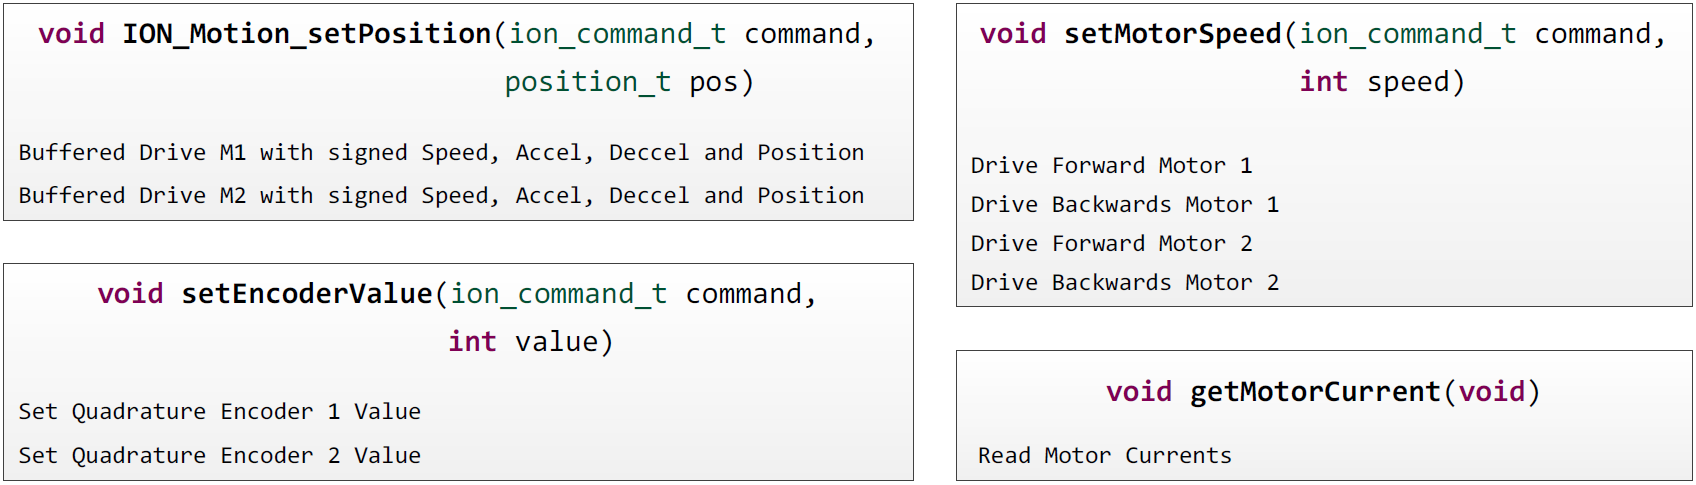
\includegraphics[width=1\textwidth]{Illustrationen/6-Umsetzung/ION_Funktionen.png}
	\caption{Software, ION Motion Driver Methoden}
	\label{fig:ION_Methoden}
\end{figure}

Auf Basis dieser vier Methoden wurde die Ansteuerung der Motoren für die Vereinzelung und die Verstellmechanik implementiert. Die beiden Prozesse sind in den Kapiteln Vereinzelung (\ref{sec:Vereinzelung}) und Verstellmechanik (\ref{verstellmechanik}) systematisch beschrieben. Die genaue Implementierung der vier Methoden kann im ION\_Motion\_Driver.c File im Anhang nachgeschlagen werden. Im folgenden Absatz wird noch kurz auf die Auswertung der mit dem Motorcontroller gemessen Motorstromwerte eingegangen.\newline
Für die Initialisierung der Verstellmechanik wird der Motor langsam in eine Richtung gedreht bis die Welle an den mechanischen Anschlag läuft. In diesem Moment steigt der Strom durch den Motor aufgrund der erhöhten Last stark an. Dieser Anstieg wird über die Auswertung der Stromwerte detektiert. Im konkreten Fall wird in der Software ein Schwellwert für die Stromstärke definiert, bei welchem der Motor angehalten soll. Um die Fluktuationen der gemessenen Stromwerte zu glätten wird ein Mittelwert über die letzten X Werte gebildet.

\begin{figure}[H]
	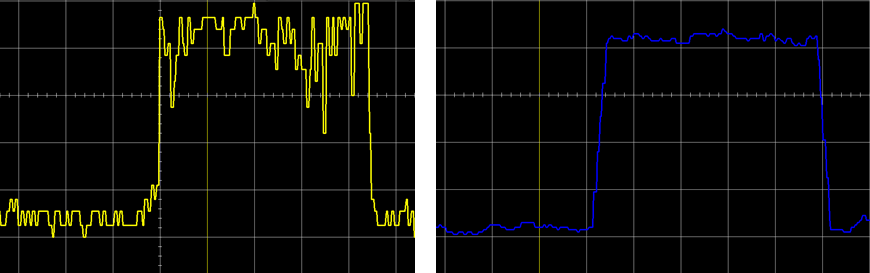
\includegraphics[width=1\textwidth]{Illustrationen/6-Umsetzung/ION_Motion_Strommessung.png}
	\caption{Software, Glättung des Motorstroms}
	\label{fig:ION_Motion_Strommessung}
\end{figure}

In Abbildung \ref{fig:ION_Motion_Strommessung} ist der Stromverlauf des Pololu Getriebemotors mit Übersetzung 378:1 abgebildet. Die Messung wurden mit der Software Segger J-Scope durchgeführt. Der Motor wurde im Leerlauf ohne Last betrieben, mit einer konstanten Last gebremst und anschliessend wieder entlastet. Dabei wurde der Motor mit einem geringen PWM Tastgrad betrieben um keinen zu grossen Laststrom zu generieren.\\
Auf den beiden Graphen ist ein deutlicher Stromanstieg zu erkennen. Der linke Graph zeigt dabei die gemessenen Stromwerte, der rechte die Mittelwerte der letzten 5 Messwerte. Der Vorteil der Mittelwertbildung kommt vor allem bei einer konstanten Belastung des Motors zum Vorschein, da hier die gemessenen Stromwerte stark fluktuieren und keine akkurate Messung zulassen. Die Stromkurven sind als qualitative Angaben zu verstehen, der Fokus liegt auf der Glättung der Messwerte.


\subsubsection{IR Sensor Driver}
Dieser Teil der Software befasst sich mit der Messgrössenerfassung und Auswertung der IR-Sensor Daten zur Topferkennung. Dabei setzt sich die Topferkennung gemäss folgender Aufzählung aus zwei Teilen zusammen:

\begin{itemize}
	\item Die Erkennung eines Topfes welcher sich vor dem Planting Robot in Position befindet um mit Nemacaps besetzt zu werden.
	\item Das Erkennen von verschiedenen Topfgrössen zur Laufzeit der Anlage. Dadurch soll sich die Verstellmechanik adaptiv an einen neuen Produktionsbatch mit anderen Töpfen anpassen.
\end{itemize}

Die Softwareauswertung der Topferkennung wurde aus Zeitgründen nicht mehr implementiert. Allerdings wurde ein Prove of Concept der Messmethode zur Erkennung der Topfposition durchgeführt. Dieses ist in Kapitel \ref{sec:Topferkennung} beschrieben.

\subsubsection{Trinamic Motion Driver}
Die Kommunikation zum Trinamic Motor Controller TMCM-1630-2C wurde über UART realisiert. Dabei beträgt die Baudrate 38400 baud. Das Command Format ist in Tabelle \ref{tab:Trinamic_Command_Format} abgebildet. Dabei ist links das Format der Commands die zum Kontroller gesendet werden und rechts die Commands die vom Kontroller zurückgesendet werden abgebildet. 

\begin{table}[H]
	\centering 
	%\subfloat[Sender]{ 
	\begin{tabular}{|c|l|}
		\hline
		\textbf{Bytes} & \textbf{Meaning} \\
		\hline
		1     & Module adress \\
		\hline
		1     & Command number \\
		\hline
		1     & Type number \\
		\hline
		1     & Motor or Bank number \\
		\hline
		4     & Value (MSB first!) \\
		\hline
		1     & Checksum \\
		\hline
	\end{tabular}%
	%}   
	\qquad 
	%\subfloat[Empfänger]{ 
	\begin{tabular}{|c|l|}
		\hline
		\textbf{Bytes} & \textbf{Meaning} \\
		\hline
		1     & Reply address \\
		\hline
		1     & Module address \\
		\hline
		1     & Status (e.g. 100 means no error) \\
		\hline
		1     & Command number \\
		\hline
		4     & Value (MSB first!) \\
		\hline
		1     & Checksum \\
		\hline
	\end{tabular}%
	%} 
	\caption{Software, Command Format Trinamic \protect\cite{Trinamic}} 
	\label{tab:Trinamic_Command_Format} 
\end{table} 

Durch die Gegebenheit, dass alle Commands welche an den Trinamic Controller geschickt werden über die gleiche Bytelänge verfügen, kann für das Senden und Empfangen von Commands jeweils eine generische Methode verwendet werden. Die beiden Methoden sind in Abb. \ref{fig:Trinamic_Funktionen} illustriert.

\begin{figure}[H]
	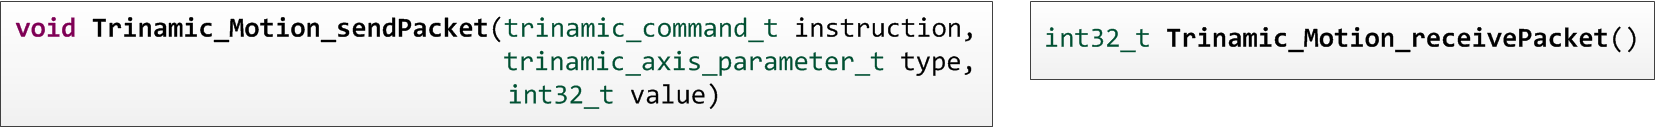
\includegraphics[width=1\textwidth]{Illustrationen/6-Umsetzung/Trinamic_Funktionen.png}
	\caption{Software, Trinamic Methoden zur Kommunikation}
	\label{fig:Trinamic_Funktionen}
\end{figure}

Um den Trinamic Motion Controller zu steuern, können über die Methode Trinamic\_Motion\_sendPacket commands zusammen mit dem jeweiligen type und einer value als Parameter mitgegeben werden. Die verwendeten commands wurden als Enum definiert und können auf diese Weise in der Software einfach verwaltet werden. Tabelle \ref{tab:Trinamic_instructions} bietet eine Übersicht über die verwendeten instructions.

\begin{table}[H]
	\centering
	\caption{Software, Trinamic Instructions Overview \protect\cite{Trinamic}}
	\begin{tabular}{|l|c|l|}
		\hline
		\textcolor[rgb]{ .247,  .247,  .247}{\textbf{Instruction}} & \textcolor[rgb]{ .247,  .247,  .247}{\textbf{Command number}} & \textcolor[rgb]{ .247,  .247,  .247}{\textbf{Meaning}} \\
		\hline
		ROR   & 1     & Rotate right \\
		\hline
		ROL   & 2     & Rotate left \\
		\hline
		MST   & 3     & Motor stop \\
		\hline
		MVP   & 4     & Move to position \\
		\hline
		SAP   & 5     & Set axis parameter \\
		\hline
		GAP   & 6     & Get axis parameter \\
		\hline
	\end{tabular}%
	\label{tab:Trinamic_instructions}%
\end{table}%

Die Commands SAP und GAP verlangen einen type Übergabeparameter welcher die Axis Parameter repräsentiert. Die axis parameter enthalten Konfigurations- sowie Statuswerte des Motion Controllers. Ein Auszug aus der Liste der verwendeten Axis Parameter ist in Tabelle \ref{tab:Trinamic_Axis_Parameter} aufgeführt.

\begin{table}[H]
	\centering
	\footnotesize
	\caption{Software, Trinamic Axis Parameter Overview \protect\cite{Trinamic}}
	\begin{tabular}{|c|l|l|l|}
		\hline
		\multicolumn{1}{|l|}{\textbf{Number}} & \textbf{Axis Parameter} & \textbf{Description} & \textbf{Access} \\
		\hline
		1     & Actual position & Set/get the position counter without moving the motor. & R / W \\
		\hline
		6     & Max current & Set/get the max allowed motor current. & R / W \\
		\hline
		11    & Acceleration & Acceleration parameter for ROL, ROR, MVP. & R / W \\
		\hline
		150   & Actual motor current & Get actual motor current. & R \\
		\hline
		172   & P current PID & P parameter of current PID regulator. & R / W \\
		\hline
		173   & I current PID & I parameter of current PID regulator. & R / W \\
		\hline
		234   & P velocity PID & P parameter of velocity PID regulator. & R / W \\
		\hline
		235   & I velocity PID & I parameter of velocity PID regulator. & R / W \\
		\hline
		230   & P position PID & P parameter of position PID regulator. & R / W \\
		\hline
	\end{tabular}
	\label{tab:Trinamic_Axis_Parameter}
\end{table}

Mit den in diesem Kapitel erläuterten Software Methoden, Commands, sowie Axis Parameter wurde der Bewegungsablauf der Setzeinheit im Trinamic\_Motion\_Driver.c File implementiert. Die entsprechenden .c und .h Files sind im Anhang zu finden.

